El Scheduler es la estructura m\'as grande y quiz\'as m\'as compleja de nuestro trabajo. Su funcion es simple, coordinar en 
que orden ocurren los eventos en nuestro Kernel y determinar ciertas acciones como si una tarea es desalojada por una operacion ilegal o mina, o un cambio simple de tareas por tick de reloj.\\
Conceptualmente nos imaginamos al Scheduler teniendo:
\begin{enumerate}
 \item Un timer llamado quantum que dictamina cuantos ciclos le queda a la corrida de tareas hasta que vuelva a empezar.
 \item Un estado pause, que en caso de estar activo hara que corra solo la tarea Idle.
 \item Un array donde guardamos el contexto de todas las tareas incluyendo la Idle.
\end{enumerate}

Corrida tarea:\\
\begin{center}
%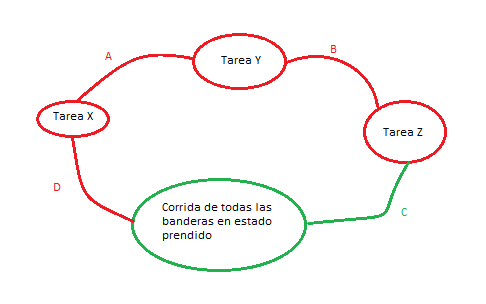
\includegraphics[scale=0.7]{imagenes/cicloBasicoTareas.png} 
\end{center}

\begin{center}
%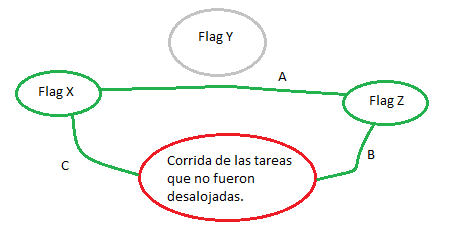
\includegraphics[scale=0.7]{imagenes/corridaFlags.png} 
\end{center}


La interrupci\'on de clock se encarga de realizar todos los saltos y cambios de tareas, exceptuando el salto a idle (que puede ser hecho 
en cualquier momento). El scheduler es la estructura que le informa hacia donde ir siguiendo. De esta forma, mantenemos el c\'odigo facilmente 
segmentado.\\

Una excepci\'on interesante es el caso en el que no querramos saltar a ningun lado sino seguir en la tarea actual. Por ejemplo, si me 
queda una sola tarea y estoy en la corrida de tareas a\'un con quantum me gustar\'ia pertenecer en esa tarea. Para esto el scheduler 
devuelve el selector de segmento 0, el cual es reconocido por el clock como una instrucci\'on para volver a la tarea anterior (iret) 
y no realizar ningun salto. (tratar de saltar a una tarea en uso daria error).
